\documentclass[12pt]{article}

\usepackage{times}
\usepackage{graphicx}
\usepackage{amsmath}
\usepackage{url}

\setlength{\textwidth}{6.5in}
\setlength{\textheight}{8.9in}
\setlength{\oddsidemargin}{0.0in}
\setlength{\topmargin}{0.05in}
\setlength{\headheight}{-0.05in}
\setlength{\headsep}{0.0in}

\newcommand{\indep}{\perp\!\!\!\perp}

\begin{document}

\begin{center}
{\bf CS 6300} \hfill {\large\bf HW08: Bayes Nets I \hfill Apr 11, 2023}
\end{center}


\section{Inference by Variable Elimination}

Consider the following Bayes' net from last week's homework. We will again derive $P(A|+e,-f)$, but this time using Variable Elimination. We will eliminate variables in the following order: D,B,C.

\begin{tabular}{cc}
\begin{tabular}{cc}
\begin{tabular}{|r|r|} \hline
A  & $P(A)$ \\ \hline
+a & 0.3      \\ \hline
-a & 0.7      \\ \hline
\end{tabular} &
\begin{tabular}{|r|r|r|} \hline
B  & A  & $P(B|A)$ \\ \hline
+b & +a & 0.7      \\ \hline
+b & -a & 0.6      \\ \hline
\end{tabular} \\[.5in]
\begin{tabular}{|r|r|r|} \hline
C  & A  & $P(C|A)$ \\ \hline
+c & +a & 0.2      \\ \hline
+c & -a & 0.9      \\ \hline
\end{tabular} &
\begin{tabular}{|r|r|r|} \hline
D  & B  & $P(D|B)$ \\ \hline
+d & +b & 0.3      \\ \hline
+d & -b & 0.4      \\ \hline
\end{tabular} \\[.5in]
\begin{tabular}{|r|r|r|} \hline
E  & C  & $P(E|C)$ \\ \hline
+e & +c & 0.4      \\ \hline
+e & -c & 0.5      \\ \hline
\end{tabular} &
\begin{tabular}{|r|r|r|} \hline
F  & C  & $P(F|C)$ \\ \hline
-f & +c & 0.9      \\ \hline
-f & -c & 0.2      \\ \hline
\end{tabular}
\end{tabular} & 
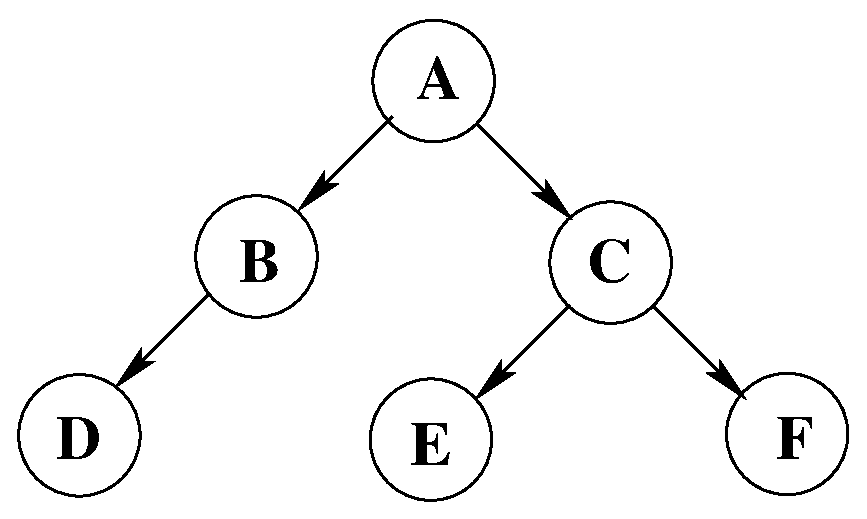
\includegraphics[height=1.5in]{ABCDEF.eps}
\end{tabular}

\vspace{0.5cm}
We have 
$$P(A|+e,-f) \propto P(A,+e,-f) = \sum_{B,C,D} P(A,B,C,D,+e,-f)$$

From the Bayes' net,

$$P(A,B,C,D,+e,-f) = P(A) P(B|A) P(C|A) P(D|B) P(+e|C) P(-f|C)$$

As a reminder, the order in which you should perform variable elimination is D,B,C. Also note that if after marginalization, all entries are 1, then you can ignore the resulting factor in all subsequent joins since it won't have any effect.

To make this more clear, let's walk through the first variable elimination and marginalization.

We start with D. The only factor involving D is $P(D|B)$. We can ignore the resulting factor, $f_1$, since after marginalization we just have ones and any joins that involve $f_1$ won't be changed by joining with $f_1$ since we will just multiple entries by 1.

\begin{tabular}{|r|r|r|} \hline
D  & B  & $P(D|B)$ \\ \hline
+d & +b & 0.3      \\ \hline
-d & +b & 0.7      \\ \hline
+d & -b & 0.4      \\ \hline
-d & -b & 0.6      \\ \hline
\end{tabular} Sum over D
\begin{tabular}{|r|r|r|} \hline
 B  & $f_1(\cdot|B)$ \\ \hline
+b & 1      \\ \hline
 -b & 1      \\ \hline
\end{tabular}\\

Continue and finish solving for $P(A|+e,-f)$ by next eliminating variable B and finally C. Then normalize.
You should be the same answer you got for HW 7. And hopefully, you'll agree that Variable Elimination is much better than full enumeration.

We're now at $$P(A|+e,-f) \propto P(A,+e,-f) = \sum_{B,C} P(A,B,C,+e,-f)$$

The next variable to eliminate is B. Since we're ignoring $f_1(\cdot|B)$, the only term that includes B is $P(B|A)$. We need to do some operations to remove this variable, a join and a summing out. Let's do the join:

\begin{tabular}{|r|r|r|} \hline
B  & A  & $P(B|A)$ \\ \hline
+b & +a & 0.7      \\ \hline
+b & -a & 0.6      \\ \hline
-b & +a & 0.3      \\ \hline
-b & -a & 0.4      \\ \hline
\end{tabular} Sum over B
\begin{tabular}{|r|r|r|} \hline
 A  & $P()$ \\ \hline
+a & 1      \\ \hline
-a & 1      \\ \hline
\end{tabular}\\

Since this factor is also all 1s, we can ignore it.

Now we're at$$P(A|+e,-f) \propto P(A,+e,-f) = \sum_{C} P(A,C,+e,-f)$$

Let's join on C and sum it out:

\begin{tabular}{|r|r|r|r|r|} \hline
A  & C  & +e & -f  & $P(A,C,+e,-f)$ \\ \hline
+a & +c & +e & -f & 0.3 * 0.2 * 0.4 * 0.9 = 0.0216  \\ \hline
+a & -c & +e & -f & 0.3 * 0.8 * 0.5 * 0.2 = 0.024   \\ \hline
-a & +c & +e & -f & 0.7 * 0.9 * 0.4 * 0.9 = 0.2268  \\ \hline
-a & -c & +e & -f & 0.7 * 0.1 * 0.5 * 0.2 = 0.007   \\ \hline
\end{tabular}Sum over C
\begin{tabular}{|r|r|r|} \hline
 A  & $P(A,+e,-f)$ \\ \hline
+a &  0.0456     \\ \hline
-a &  0.2338     \\ \hline
\end{tabular}\\

Now normalizing, we get:
\begin{tabular}{|r|r|r|} \hline
 A  & $P(A,+e,-f)$ \\ \hline
+a &  0.1632    \\ \hline
-a &  0.8368    \\ \hline
\end{tabular}\\



\clearpage

\section{Sampling}

Consider the Bayes net below with corresponding CPTs.  

\begin{enumerate}

\item Generate 2 samples using the following random numbers for the following nodes:

\begin{center}
\begin{tabular}{|c|c|c|c|c|c|c|c|c|c|} \hline
A & B & C & D & A & B & C & D \\
0.31 & 0.58 & 0.04 & 0.94 & 0.67 & 0.49 & 0.37 & 0.42 \\ \hline
\end{tabular}
\end{center}

\begin{center}
\begin{tabular}{cc}
\begin{tabular}{cccc}
\begin{tabular}{|c|c|} \hline
A  & P(A) \\ \hline
+a & 0.8  \\ \hline
-a & 0.2  \\ \hline
\end{tabular} & 
\begin{tabular}{|r|r|r|} \hline
A  & B  & $P(B|A)$ \\ \hline
+a & +b & 0.8  \\ \hline
+a & -b & 0.2  \\ \hline
-a & +b & 0.5  \\ \hline
-a & -b & 0.5  \\ \hline
\end{tabular} \\[.4in]
\begin{tabular}{|r|r|r|} \hline
A  & C  & $P(C|A)$ \\ \hline
+a & +c & 0.7  \\ \hline
+a & -c & 0.3  \\ \hline
-a & +c & 0.1  \\ \hline
-a & -c & 0.9  \\ \hline
\end{tabular} &
\begin{tabular}{|r|r|r|r|} \hline
B  & C  & D  & $P(D|B,C)$ \\ \hline
+b & +c & +d & 0.3      \\ \hline
+b & +c & -d & 0.7      \\ \hline
+b & -c & +d & 0.1      \\ \hline
+b & -c & -d & 0.9      \\ \hline
-b & +c & +d & 0.2      \\ \hline
-b & +c & -d & 0.8      \\ \hline
-b & -c & +d & 0.9      \\ \hline
-b & -c & -d & 0.1      \\ \hline
\end{tabular}
\end{tabular} & 
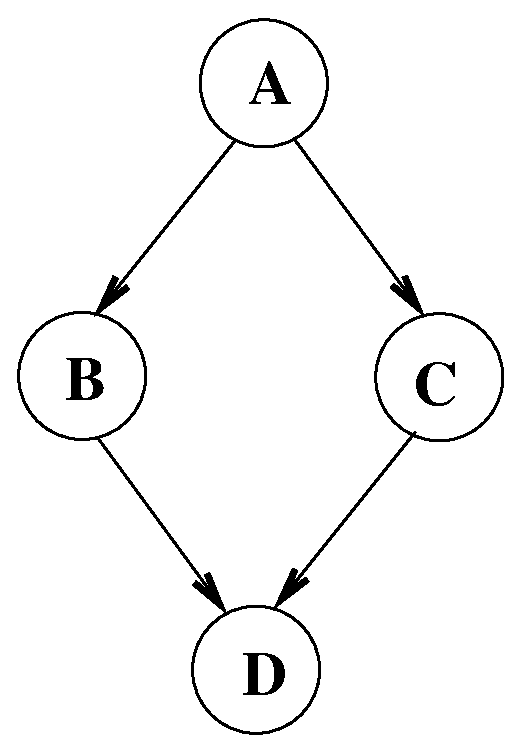
\includegraphics[height=2in]{ABCD.eps}
\end{tabular}
\end{center}

The samples are:

\begin{flushleft}
\begin{tabular}{llll}
+a & +b & +c & -d \\
+a & +b & +c & -d \\
\end{tabular}
\end{flushleft}

\item Given the samples below, answer the subsequent queries. We've done the first one for you.

\begin{flushleft}
\begin{tabular}{rrrrr} 
+a & -b & -c & -d  \\
-a & +b & +c & -d  \\
+a & -b & +c & -d  \\
+a & +b & -c & -d  \\
+a & -b & +c & +d  \\
-a & -b & -c & +d  \\
-a & -b & -c & -d  \\
+a & +b & +c & -d  \\
-a & +b & -c & -d  \\
+a & +b & -c & +d  \\
\end{tabular}
\end{flushleft}

\begin{enumerate}

  \item $P(+d) = 3/10$

  \item $P(+a,-b) = 3/10$

  \item $P(-a,-b,-c,-d) = 1/10$

  \item $P(+d | -a, -b) = 1/2$

\end{enumerate}

\item Consider the query $P(-d|-a,-b)$.  Using the following random numbers, generate samples and their weights using likelihood
  weighting.

\begin{center}
\begin{tabular}{|c|c|c|c|c|c|c|c|c|c|} \hline
0.31 & 0.58 & 0.89 & 0.15  \\ \hline
\end{tabular}
\end{center}

The samples and weights are:

\begin{flushleft}
\begin{tabular}{rrrrr}
-a & -b & -c & +d & ?\\
-a & -b & -c & +d & ?\\
\end{tabular}
\end{flushleft}

\item Given the weighted samples below, answer the subsequent queries. We've done the first one for you.

\begin{flushleft}
\begin{tabular}{rrrrr} 
+a & -b & -c & -d & 0.3 \\
-a & +b & +c & -d & 0.4 \\
+a & -b & +c & -d & 0.1 \\
+a & +b & -c & -d & 0.3 \\
+a & -b & +c & +d & 0.4 \\
-a & -b & -c & +d & 0.1 \\
-a & -b & -c & -d & 0.2 \\
+a & +b & +c & -d & 0.5 \\
-a & +b & -c & -d & 0.7 \\
+a & +b & -c & +d & 0.8 \\
\end{tabular}
\end{flushleft}

\begin{enumerate}

  \item $P(+d) = (0.4+0.1+0.8)/(0.3+0.4+0.1+0.3+0.4+0.1+0.2+0.5+0.7+0.8) = 1.3/3.8$

  \item $P(+a,-b) = (0.3+0.1+0.4)/(0.3+0.4+0.1+0.3+0.4+0.1+0.2+0.5+0.7+0.8) = 0.8/3.8$

  \item $P(-a,-b,-c,-d) = (0.2)/(0.3+0.4+0.1+0.3+0.4+0.1+0.2+0.5+0.7+0.8) = 0.2/3.8$

  \item $P(+d | -a, -b) = (0.1)/(0.1+0.2) = 0.1/0.3 $

\end{enumerate}

\end{enumerate}



\end{document}